\chapter*{}
%\thispagestyle{empty}
%\cleardoublepage

%\thispagestyle{empty}

\begin{titlepage}
 
 
\setlength{\centeroffset}{-0.5\oddsidemargin}
\addtolength{\centeroffset}{0.5\evensidemargin}
\thispagestyle{empty}

\noindent\hspace*{\centeroffset}\begin{minipage}{\textwidth}

\centering
%
\includegraphics[width=0.9\textwidth]{imagenes/logo_ugr.jpg}\\[1.4cm]

%\textsc{ \Large PROYECTO FIN DE CARRERA\\[0.2cm]}
%\textsc{ INGENIERÍA EN INFORMÁTICA}\\[1cm]
% Upper part of the page
% 

 \vspace{3.3cm}

%si el proyecto tiene logo poner aquí
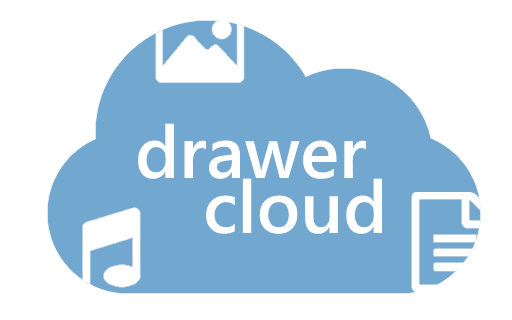
\includegraphics[width=1\textwidth]{imagenes/logo.png} 
 \vspace{0.5cm}

% Title

{\Huge\bfseries drawercloud\\
}
\noindent\rule[-1ex]{\textwidth}{3pt}\\[3.5ex]
{\large\bfseries Aplicación web orientada al almacenamiento de archivos en la nube.\\[4cm]}
\end{minipage}

\vspace{2.5cm}
\noindent\hspace*{\centeroffset}\begin{minipage}{\textwidth}
\centering

\textbf{Autor}\\ {José Manuel Rejón Santiago (alumno)}\\[2.5ex]
\textbf{Director}\\
{Prof. Dr. José María Guirao Miras}\\[2cm]
%
\includegraphics[width=0.15\textwidth]{imagenes/tstc.png}\\[0.1cm]
%\textsc{Departamento de Teoría de la Señal, Telemática y Comunicaciones}\\
%\textsc{---}\\
%Granada, mes de 201
\end{minipage}
%\addtolength{\textwidth}{\centeroffset}
\vspace{\stretch{2}}

 
\end{titlepage}




\clearpage
\thispagestyle{empty}

\begin{center}
{\large\bfseries drawercloud: aplicación web orientada al almacenamiento de archivos en la nube}\\
\end{center}
\begin{center}
José Manuel Rejón Santiago (alumno)\\
\end{center}

%\vspace{0.7cm}
\noindent{\textbf{Palabras clave}: aplicación web, cloud, pc, tablet, smartphone, servidor web}\\

\vspace{0.5cm}
\noindent{\textbf{Resumen}}\\

\textbf{drawercloud} es una aplicación web para el alojamiento de archivos en la nube (cloud). Los usuarios podrán realizar diversas tareas sobre sus archivos, como por ejemplo: Añadir/Eliminar archivos en la nube, reproducir archivos multimedia, organizar archivos en directorios, compartir archivos, descargar en un dispositivo (pc, tablet, smartphone)... De este modo, conseguiremos tener nuestros archivos almacenados en un servidor web, ahorrando espacio en nuestros dispositivos y con la seguridad de tener nuestro material a salvo en otro lugar.\\

\clearpage


\thispagestyle{empty}


\begin{center}
{\large\bfseries drawercloud: aplicación web orientada al almacenamiento de archivos en la nube}\\
\end{center}
\begin{center}
José Manuel Rejón Santiago (student)\\
\end{center}

%\vspace{0.7cm}
\noindent{\textbf{Keywords}: web application, cloud, pc, tablet, smartphone, web server}\\

\vspace{0.7cm}
\noindent{\textbf{Abstract}}\\

drawecloud is a web application for file hosting in the cloud. The users can work with their files, for example: add/delete files in the cloud, play multimedia files, organize the files in different directories, share files, download to devices (pc, tablet, smartphone)... With this, we'll achieve the task of having all our files stored in a web server, saving space in our devices and with the security of having eveything safe in another place.

\chapter*{}
\thispagestyle{empty}

\noindent\rule[-1ex]{\textwidth}{2pt}\\[4.5ex]

Yo, \textbf{José Manuel Rejón Santiago}, alumno de la titulación Grado en Ingeniería Informática de la \textbf{Escuela Técnica Superior
de Ingenierías Informática y de Telecomunicación de la Universidad de Granada}, con DNI 20077299R, autorizo la
ubicación de la siguiente copia de mi Trabajo Fin de Grado en la biblioteca del centro para que pueda ser
consultada por las personas que lo deseen.

\vspace{6cm}

\noindent Fdo: José Manuel Rejón Santiago

\vspace{2cm}

\begin{flushright}
Granada a 12 de Septiembre de 2017.
\end{flushright}


\chapter*{}
\thispagestyle{empty}

\noindent\rule[-1ex]{\textwidth}{2pt}\\[4.5ex]

D. \textbf{Prof. Dr. José María Guirao Miras (tutor)}, Profesor del Departamento de Lenguajes y Sistemas Informáticos de la Universidad de Granada.

\vspace{0.5cm}

\textbf{Informan:}

\vspace{0.5cm}

Que el presente trabajo, titulado \textit{\textbf{drawercloud, aplicación web orientada al almacenamiento de archivos en la nube}},
ha sido realizado bajo su supervisión por \textbf{José Manuel Rejón Santiago (alumno)}, y autoriza la defensa de dicho trabajo ante el tribunal
que corresponda.

\vspace{0.5cm}

Y para que conste, expiden y firman el presente informe en Granada a 12 de Septiembre de 2017.

\vspace{1cm}

\textbf{El tutor:}

\vspace{5cm}

\noindent \textbf{Prof. Dr. José María Guirao Miras}

\chapter*{Agradecimientos}
\thispagestyle{empty}

       \vspace{1cm}


En primer lugar quiero mostrar mi agradecimiento a mi tutor José María Guirao Miras por darme la oportunidad de realizar este proyecto y toda la ayuda y consejos recibidos. \\

También agradecer a mi familia y amigos/as que han estado apoyándome durante todo el desarrollo del proyecto como a lo largo de estos años de carrera. \\

Por último y no menos importante a mis compañeros durante esta experiencia, un gran apoyo siempre tanto dentro como fuera de clase.



